% Frames removed from the L14a deck on 2026-11-23, when the section "Updating the Single Index Model"
% moved to L15a. Staged for the L15a deck; this file is NOT built on its own.
% Figure paths point to ../figs/Fig-L15a-*.pdf. The \repo macro must point to
% https://github.com/varnerlab/CHEME-5660-CourseRepository-Fall-2026/blob/main/lectures/week-15/L15a
% Not yet synced with the L15a lecture: the extension "Updating the General Factor Model" has no frame.

% ========== Updating the single index model
\begin{frame}{Updating the Single Index Model}
  A stock's market sensitivity changes over time. By late 2026, most stocks in our universe moved
  less with the market than their 2014 to 2024 estimates say:
  \begin{center}
    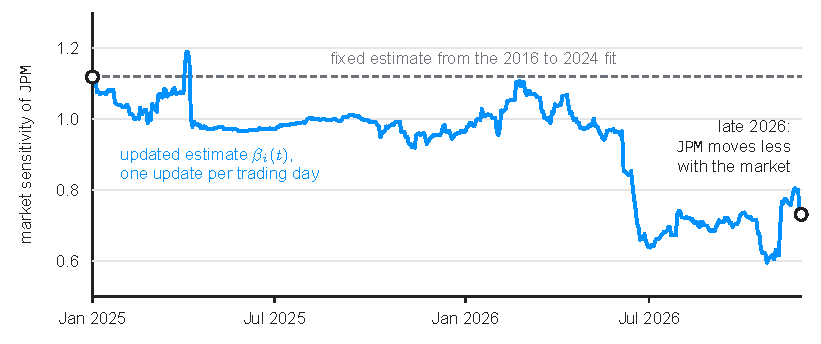
\includegraphics[width=\textwidth,height=0.53\textheight,keepaspectratio]{../figs/Fig-L15a-EWLS-JPM.pdf}
  \end{center}
  We keep the estimates current by updating them with each new trading day, giving recent days
  the most weight.
\end{frame}

\begin{frame}{Exponentially Weighted Least Squares (EWLS)}
  Previously, we estimated $\alpha_{i}$ and $\beta_{i}$ by least squares, where we minimized the
  sum of squared residuals with every training day counted the same.

  \vspace{0.6em}
  However, we could include \hilite{new information} as it arrives by weighting the new days more
  than the old ones. Let's consider exponentially weighted least squares (EWLS).
\end{frame}

\begin{frame}{The EWLS Problem}
  On day $t$, the updated baseline $\alpha_{i}(t)$ and market sensitivity $\beta_{i}(t)$ of stock
  $i$ solve:
  \begin{equation*}
    \left(\alpha_{i}(t),\beta_{i}(t)\right)=\arg\min_{\alpha_{i},\,\beta_{i}}\Biggl[\underbrace{\sum_{k=1}^{t}\phi^{\,t-k}\,\bigl(\overbrace{g_{i}(k)-\alpha_{i}-\beta_{i}\,g_{m}(k)}^{\textstyle\text{residual }r_{i}(k)}\bigr)^{2}}_{\textstyle\text{new days}}+\underbrace{\phi^{\,t}\,\frac{N_{0}}{2766}\sum_{k=-2765}^{0}r_{i}(k)^{2}}_{\textstyle\text{prior}}\Biggr]
  \end{equation*}
  where $g_{i}(k)$ and $g_{m}(k)$ are the daily growth rates of stock $i$ and \texttt{SPY} (1/yr).
  Day $0$ is December 31, 2024, the
  last day of the 2014 to 2024 fit, day $1$ is January 2, 2025, and day $469$ is November 13, 2026,
  the last day of our data.

  \vspace{0.6em}
  The implementation updates the estimates from a few running sums.
  \slidenote{Derivation:}{\href{\repo/advanced/ewls/CHEME-5660-L15a-Derivation-EWLS-Update-Fall-2026.ipynb}{The EWLS recursion (advanced notebook)}.}
\end{frame}

\begin{frame}{The Parts of the Update}
  \begin{itemize}\setlength{\itemsep}{0.6em}
    \item \hilite{New days}: day $k$ has the weight $\phi^{\,t-k}$, the decay
      $\phi=2^{-1/63}\approx 0.989$ raised to the day's age. On day $3$, January 6, 2025, the
      first sum is $\phi^{2}\,r_{i}(1)^{2}+\phi\,r_{i}(2)^{2}+r_{i}(3)^{2}$. The weight halves every 63
      trading days, about three months.
    \item \hilite{Prior}: each of the 2,766 days of 2014 to 2024 gets the weight $N_{0}/2766$, with
      $N_{0}=63$. On day $0$, the prior alone gives the 2014 to 2024 fit. After that, the factor
      $\phi^{\,t}$ shrinks the prior's day $0$ weight.
    \item \hilite{No look-ahead}: day $t$ uses the growth rates through day $t$. The trading
      method decides after the close and trades at the next open. However, this is still a
      backward-looking estimate.
  \end{itemize}
\end{frame}

\begin{frame}{Preference Weights with Updated Estimates}
  Previously, we computed the preference weight $\gamma_{i}(t)$ of each stock and used it to rank
  the stocks. The preference weight depends on the market state $\xi_{t}$, which compares a 21-day
  and a 63-day EMA of the \texttt{SPY} price:
  \begin{equation*}
    \xi_{t}=-G\left(\frac{\bar{S}^{\text{short}}_{t}}{\bar{S}^{\text{long}}_{t}}-1\right)
  \end{equation*}
  where the gain $G>0$ scales $\xi_{t}$ so that $|\xi_{t}|\leq 1$ on 99\% of training days.

  \vspace{0.5em}
  When the market falls, recent prices sit below the quarter's average, and $\xi_{t}$ turns
  positive. The day $\xi_{t}$ changes sign is a \hilite{market turn}, the regime change that the
  trading method acts on.
\end{frame}

\begin{frame}{Pick Days}
  The estimates and the preference weights update every trading day, but the basket of stocks we
  hold changes only on pick days:
  \begin{center}
    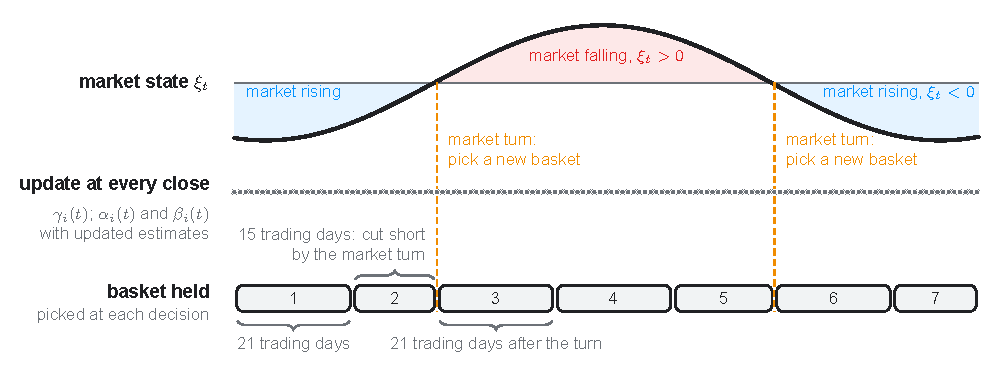
\includegraphics[width=\textwidth,height=0.56\textheight,keepaspectratio]{../figs/Fig-L15a-Gamma-Picks.pdf}
  \end{center}
  The trading method of \href{https://arxiv.org/abs/2611.03022}{Varner (2026)} picks its stocks
  with this preference weight.
\end{frame}

\begin{frame}{The Preference Model with Updated Estimates}
  For stock $i$ on day $t$, the preference weight is given by:
  \begin{equation*}
    \boxed{\begin{aligned}
      \gamma_{i}(t)&=\tanh\left(h\,\frac{\tilde{g}_{i,t}}{\max\left(|\beta_{i}(t)|,\,\beta_{\text{floor}}\right)^{\xi_{t}}}\right)\\
      &=\tanh\left(h\,\frac{\alpha_{i}(t)+\beta_{i}(t)\,\tilde{g}_{M,t}}{\max\left(|\beta_{i}(t)|,\,\beta_{\text{floor}}\right)^{\xi_{t}}}\right)
    \end{aligned}}
  \end{equation*}
  where $\tilde{g}_{i,t}$ is the expected growth rate of stock $i$ in today's market (1/yr), the
  horizon is $h=1$ year, and the floor is $\beta_{\text{floor}}=0.1$. With a fixed
  $\beta_{i}\geq\beta_{\text{floor}}$, this is the preference weight we used before.

  \vspace{0.4em}
  The second line uses the single index model, where $\tilde{g}_{M,t}$ (1/yr) is a 252-day EMA of
  the market growth rates. A different factor model, or the stock's past growth rates alone,
  could give $\tilde{g}_{i,t}$ instead.
\end{frame}

\begin{frame}{The Trading Method Makes Three Changes}
  \begin{itemize}\setlength{\itemsep}{0.6em}
    \item \hilite{Updated estimates}: $\alpha_{i}(t)$ and $\beta_{i}(t)$ come from the daily EWLS
      update, so the preference weight follows the changes in each stock's market sensitivity.
      AQR's \href{https://www.aqr.com/Insights/Research/Journal-Article/Betting-Against-Beta}{betting-against-beta portfolio}
      also re-estimates the market sensitivity of each stock from a rolling window of past returns.
    \item \hilite{A floor on the market sensitivity}: some stocks have an updated market
      sensitivity near or below zero. The denominator uses $|\beta_{i}(t)|$ with a floor, which
      keeps the denominator positive for every stock. The sign of the preference weight is then
      the sign of $\tilde{g}_{i,t}$.
    \item \hilite{Picks at market turns}: the \hilite{preference basket} holds the stocks with the
      highest preference weights in each sector, and we choose how many to keep. The method picks
      a new basket every 21 trading days and whenever the market turns, but other triggers are
      also possible.
  \end{itemize}
\end{frame}

\begin{frame}{The Market Hedge}
  The trading method can also run with a \hilite{market hedge}, which limits the market
  sensitivity of the whole portfolio. The limit drops as the market falls:
  \begin{center}
    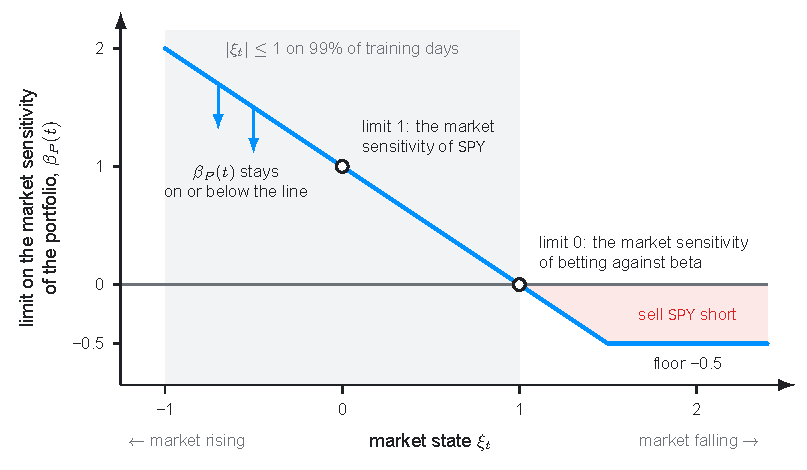
\includegraphics[width=\textwidth,height=0.6\textheight,keepaspectratio]{../figs/Fig-L15a-Market-Hedge.pdf}
  \end{center}
  Because $|\xi_{t}|\leq 1$ on 99\% of training days, only a steep fall takes the limit below zero.
\end{frame}

\begin{frame}{The Market Hedge Limit}
  On each day $t$ that the trading method sets its holdings, the hedge requires:
  \begin{equation*}
    \boxed{\beta_{P}(t)=\sum_{i}w_{i}(t)\,\beta_{i}(t)\leq\max\left(1-\xi_{t},\,-0.5\right)}
  \end{equation*}
  where $w_{i}(t)$ is the fraction of the portfolio's value in holding $i$, negative for a short.
  \begin{itemize}\setlength{\itemsep}{0.2em}
    \item \hilite{Market rise} ($\xi_{t}<0$): the limit is above one. With no borrowing,
      $\beta_{P}(t)$ rises above one only when the stocks held move more than the market.
    \item \hilite{Flat or falling market} ($0\leq\xi_{t}\leq 1$): the limit drops from one, the
      market sensitivity of \texttt{SPY}, to zero. The method shifts value
      toward low-sensitivity stocks, holds cash, or buys up to five stocks whose market sensitivity
      is zero or negative.
    \item \hilite{Steep fall} ($\xi_{t}>1$): the stocks and cash are uncorrelated or anti-correlated
      with the market, and a \texttt{SPY} short worth 20\% of the portfolio lowers $\beta_{P}(t)$ by
      $0.2$. The floor of $-0.5$ caps the short at half of the portfolio's value.
  \end{itemize}
\end{frame}

\begin{frame}{The Trading Method and Betting Against Beta}
  \vspace{0.05em}
  {\large\textbf{\ink{How does the trading method compare with betting against beta?}}}

  \vspace{0.2em}
  Previously, we met \href{https://www.aqr.com/Our-Firm/About-Us}{AQR Capital Management}, where Andrea
  Frazzini and Lasse H. Pedersen proposed the
  \href{https://www.aqr.com/Insights/Research/Journal-Article/Betting-Against-Beta}{betting-against-beta portfolio}
  in 2014. Their portfolio always buys stocks with a low market sensitivity and sells stocks with
  a high one, in amounts that make its market sensitivity zero. The trading method makes the same
  bet only when the market falls:

  \vspace{0.05em}
  \begin{itemize}\setlength{\itemsep}{0.15em}
    \item \hilite{Signal}: when the market falls ($\xi_{t}>0$), the preference weight favors stocks
      with a positive expected growth rate that move less with the market. When the market rises ($\xi_{t}<0$), the tilt reverses.
    \item \hilite{Long-only basket}: the preference basket keeps the stocks with the highest
      preference weights in each sector. A low-weight stock is left out, not sold short.
    \item \hilite{Market hedge}: at $\xi_{t}=1$, the limit on $\beta_{P}(t)$ is zero, the market
      sensitivity of betting against beta. Betting against beta gets there by selling stocks with a
      high market sensitivity. The method sells only \texttt{SPY} short, after a steeper fall.
  \end{itemize}
\end{frame}

\begin{frame}{Example: Updating the Single Index Model}
  \vspace{0.3em}
  {\normalsize\textbf{\ink{Review on your own:}}\par\small
  \href{\repo/CHEME-5660-L15a-Example-Updating-SIM-Gamma-Fall-2026.ipynb}{\dimmed{CHEME-5660-L15a-Example-Updating-SIM-Gamma-Fall-2026.ipynb}}}

  \vspace{0.8em}
  In this example, we update the single index model of every stock with each trading day of 2025
  and 2026, starting from the 2014 to 2024 fit. We pick the preference basket once a month and
  whenever the market turns, and compare it with the basket that the fixed estimates pick.

  \vspace{0.8em}
  for the stocks of a basket to a paper trading account.
\end{frame}

% ========== Optional advanced material
\begin{frame}{Optional Advanced Material}
  \vspace{0.2em}
  {\normalsize\textbf{\ink{The daily update of the single index model:}} \dimmed{advanced/ewls/}\par
  \href{\repo/advanced/ewls/CHEME-5660-L15a-Derivation-EWLS-Update-Fall-2026.ipynb}{\dimmed{CHEME-5660-L15a-Derivation-EWLS-Update-Fall-2026.ipynb}}}

  \vspace{0.3em}
  We derive the running sums that the exponentially weighted least squares update carries from
  one day to the next. We solve them for the updated estimates and the residual standard deviation,
  and show how the 2014 to 2024 fit seeds the sums.
\end{frame}
